\documentclass[12pt,a4paper]{report}

% Packages
\usepackage[utf8]{inputenc}
\usepackage[T1]{fontenc}
\usepackage[english]{babel}
\usepackage{amsmath,amssymb,amsfonts}
\usepackage{graphicx}
\usepackage{booktabs}
\usepackage{longtable}
\usepackage{hyperref}
\usepackage{listings}
\usepackage{xcolor}
\usepackage{subcaption}
\usepackage{multirow}
\usepackage[margin=2.5cm]{geometry}
\usepackage{float}
\usepackage{enumitem}
\usepackage{tikz}
\usetikzlibrary{arrows.meta,positioning,shapes.geometric,fit,calc}
\usepackage{tcolorbox}
\usepackage{xcolor}
\usepackage{mdframed}

% TikZ libraries for advanced diagrams
\usetikzlibrary{patterns,backgrounds,decorations.pathreplacing}
\usetikzlibrary{mindmap,trees,decorations.text}
\usetikzlibrary{matrix,chains,scopes}
\usetikzlibrary{decorations.pathmorphing,shapes.symbols}

% Color definitions for consistent theming
\definecolor{tumorcell}{RGB}{220,20,60}
\definecolor{immunecell}{RGB}{30,144,255}
\definecolor{bloodvessel}{RGB}{255,69,0}
\definecolor{glucose}{RGB}{255,215,0}
\definecolor{dna}{RGB}{138,43,226}
\definecolor{treatment}{RGB}{34,139,34}

\begin{document}

\chapter{Theoretical Background}
\label{ch:theoretical_background}

Understanding why traditional mathematical approaches fail to capture cancer's complexity is the first step toward building better models. This chapter reveals why agent-based modeling succeeds where differential equations struggle --- and lays the foundation for a virtual tumor that behaves like real biology.

This chapter presents the theoretical foundations upon which the RCC agent-based model is constructed. We begin with a formal introduction to agent-based modeling and the Repast4Py framework, then review the immunology of renal cell carcinoma with emphasis on the cell types represented in the model, discuss the metabolic characteristics of the tumor microenvironment, and conclude with an overview of the treatment modalities implemented in the simulation.

% ============================================================================
\section{Agent-Based Modeling}
\label{sec:bg_abm}
% ============================================================================

An agent-based model (ABM) consists of autonomous agents, a shared environment, and behavioral rules. The distinguishing feature is that system-level behavior is emergent: it arises from the aggregate of individual agent actions and interactions rather than being prescribed by global equations. This makes ABM particularly powerful for systems characterized by heterogeneity, spatial structure, and nonlinear feedback—properties that are hallmarks of the tumor microenvironment.

ABM offers several advantages for biological systems: heterogeneity (each cell carries unique properties like DNA sequences), spatial dynamics (3D grid positions determine which cells can interact), stochasticity (biological events are inherently probabilistic), and modularity (new agent types or environmental layers can be added without restructuring the entire model).

Repast4Py is a Python-based agent-based modeling framework leveraging MPI for parallel simulations. Key abstractions include Agent (base class), SharedContext (distributed agent container), and SharedGrid (spatial projection) with sticky boundaries and multiple occupancy support.

\begin{figure}[htbp]
\centering
\adjustbox{max width=0.85\textwidth, max height=0.7\textheight}{% ABM vs ODE/PDE Comparison Diagram
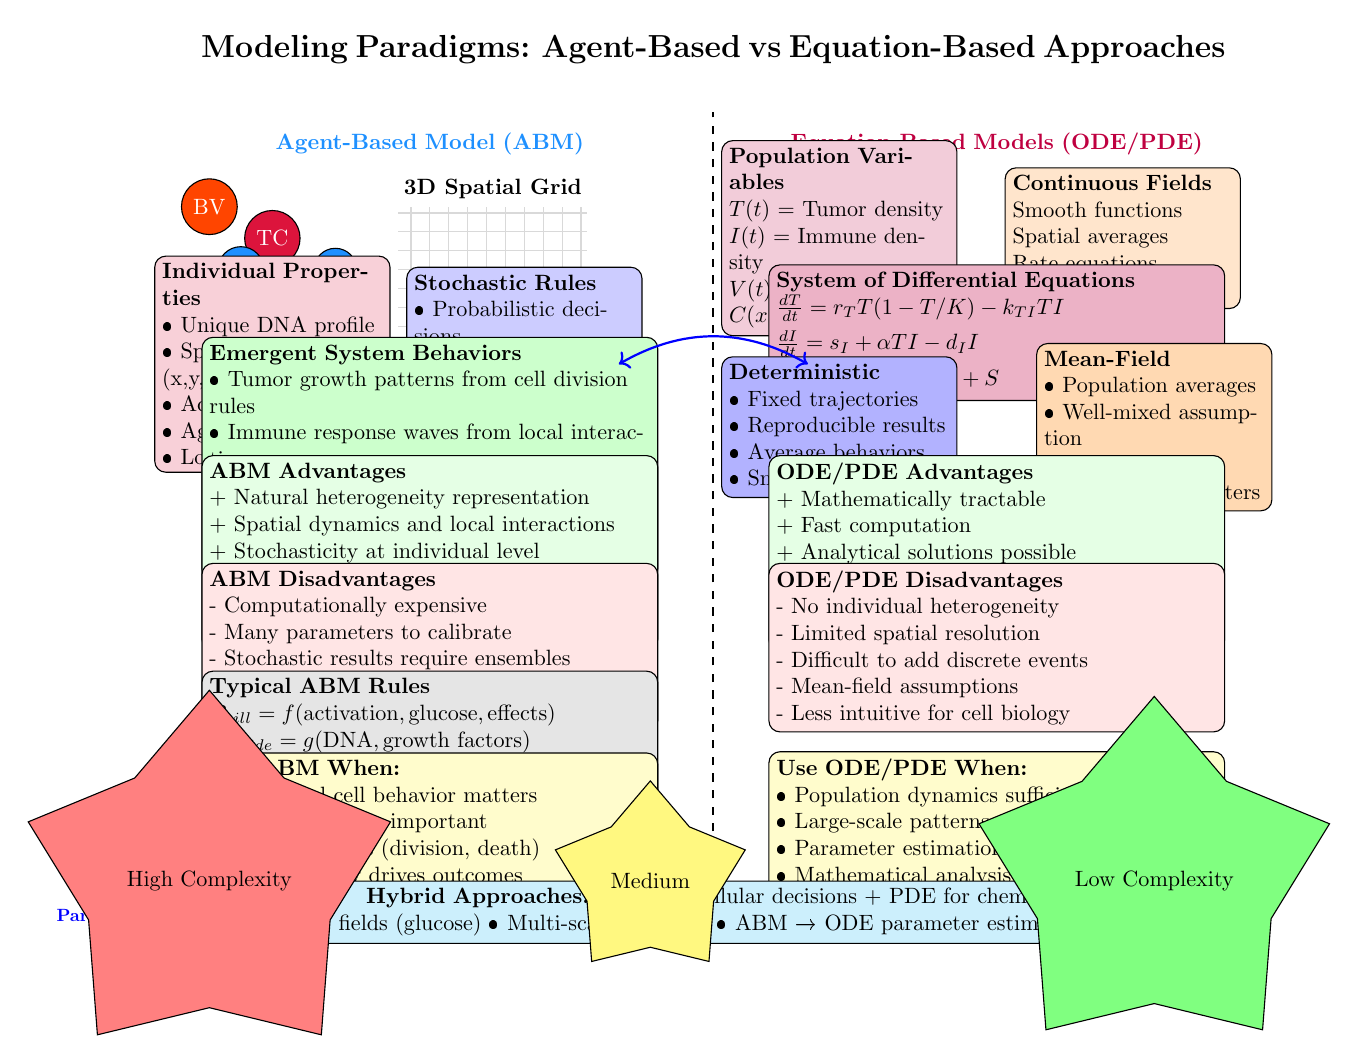
\begin{tikzpicture}[scale=0.8, every node/.style={scale=0.8}]

% Title
\node[text width=18cm, text centered] at (9,14) {
    \Large\textbf{Modeling Paradigms: Agent-Based vs Equation-Based Approaches}
};

% Divide into two sides
\draw[thick, dashed] (9,0) -- (9,13);

% ABM Side (Left)
\node[text width=8cm, text centered] at (4.5,12.5) {\textbf{\textcolor{immunecell}{Agent-Based Model (ABM)}}};

% Individual agents
\node[draw, circle, fill=tumorcell, text=white, minimum size=0.8cm] at (2,11) {TC};
\node[draw, circle, fill=immunecell, text=white, minimum size=0.6cm] at (3,10.5) {T};
\node[draw, circle, fill=immunecell, text=white, minimum size=0.6cm] at (1.5,10.5) {M};
\node[draw, circle, fill=immunecell, text=white, minimum size=0.6cm] at (2.5,10) {NK};
\node[draw, circle, fill=bloodvessel, text=white, minimum size=0.6cm] at (1,11.5) {BV};

% Grid representation
\draw[step=0.3cm, gray!30] (4,9.5) grid (7,11.5);
\node[above] at (5.5,11.5) {\textbf{3D Spatial Grid}};

% Individual cell properties
\node[draw, rounded corners, fill=tumorcell!20, text width=3.5cm] at (2,9) {
    \textbf{Individual Properties}\\
    • Unique DNA profile\\
    • Spatial position (x,y,z)\\
    • Activation state\\
    • Age/lifecycle\\
    • Local interactions
};

% Stochastic rules
\node[draw, rounded corners, fill=blue!20, text width=3.5cm] at (6,9) {
    \textbf{Stochastic Rules}\\
    • Probabilistic decisions\\
    • Random movement\\
    • Bernoulli events\\
    • Monte Carlo sampling
};

% Emergent behaviors
\node[draw, rounded corners, fill=green!20, text width=7cm] at (4.5,7.5) {
    \textbf{Emergent System Behaviors}\\
    • Tumor growth patterns from cell division rules\\
    • Immune response waves from local interactions\\
    • Spatial clustering without global coordination\\
    • Treatment resistance from mutation accumulation
};

% Advantages
\node[draw, rounded corners, fill=green!10, text width=7cm] at (4.5,6) {
    \textbf{ABM Advantages}\\
    + Natural heterogeneity representation\\
    + Spatial dynamics and local interactions\\
    + Stochasticity at individual level\\
    + Easy addition of new cell types\\
    + Direct biological interpretation\\
    + Modular/extensible architecture
};

% Disadvantages
\node[draw, rounded corners, fill=red!10, text width=7cm] at (4.5,4.5) {
    \textbf{ABM Disadvantages}\\
    - Computationally expensive\\
    - Many parameters to calibrate\\
    - Stochastic results require ensembles\\
    - Difficult mathematical analysis\\
    - Scale limitations (memory/time)
};

% Example equation
\node[draw, rounded corners, fill=gray!20, text width=7cm] at (4.5,3) {
    \textbf{Typical ABM Rules}\\
    $P_{kill} = f(\text{activation}, \text{glucose}, \text{effects})$\\
    $P_{divide} = g(\text{DNA}, \text{growth factors})$\\
    $\mathbf{x}_{t+1} = \mathbf{x}_t + \text{movement}(\text{targets})$\\
    IF random() $< P_{kill}$ THEN remove target
};

% ODE/PDE Side (Right)
\node[text width=8cm, text centered] at (13.5,12.5) {\textbf{\textcolor{purple}{Equation-Based Models (ODE/PDE)}}};

% Population-level variables
\node[draw, rounded corners, fill=purple!20, text width=3.5cm] at (11,11) {
    \textbf{Population Variables}\\
    $T(t)$ = Tumor density\\
    $I(t)$ = Immune density\\
    $V(t)$ = Vessel density\\
    $C(x,t)$ = Drug conc.
};

% Continuous functions
\node[draw, rounded corners, fill=orange!20, text width=3.5cm] at (15.5,11) {
    \textbf{Continuous Fields}\\
    Smooth functions\\
    Spatial averages\\
    Rate equations\\
    Analytical solutions
};

% Differential equations
\node[draw, rounded corners, fill=purple!30, text width=7cm] at (13.5,9.5) {
    \textbf{System of Differential Equations}\\
    $\frac{dT}{dt} = r_T T(1-T/K) - k_{TI} TI$\\[0.1cm]
    $\frac{dI}{dt} = s_I + \alpha TI - d_I I$\\[0.1cm]
    $\frac{\partial C}{\partial t} = D\nabla^2 C - \lambda C + S$
};

% Deterministic dynamics
\node[draw, rounded corners, fill=blue!30, text width=3.5cm] at (11,8) {
    \textbf{Deterministic}\\
    • Fixed trajectories\\
    • Reproducible results\\
    • Average behaviors\\
    • Smooth dynamics
};

% Mean-field approximation
\node[draw, rounded corners, fill=orange!30, text width=3.5cm] at (16,8) {
    \textbf{Mean-Field}\\
    • Population averages\\
    • Well-mixed assumption\\
    • Rate constants\\
    • Effective parameters
};

% Advantages
\node[draw, rounded corners, fill=green!10, text width=7cm] at (13.5,6) {
    \textbf{ODE/PDE Advantages}\\
    + Mathematically tractable\\
    + Fast computation\\
    + Analytical solutions possible\\
    + Parameter sensitivity analysis\\
    + Stability/bifurcation analysis\\
    + Well-established theory
};

% Disadvantages
\node[draw, rounded corners, fill=red!10, text width=7cm] at (13.5,4.5) {
    \textbf{ODE/PDE Disadvantages}\\
    - No individual heterogeneity\\
    - Limited spatial resolution\\
    - Difficult to add discrete events\\
    - Mean-field assumptions\\
    - Less intuitive for cell biology
};

% When to use each
\node[draw, rounded corners, fill=yellow!20, text width=7cm] at (4.5,1.5) {
    \textbf{Use ABM When:}\\
    • Individual cell behavior matters\\
    • Spatial patterns important\\
    • Discrete events (division, death)\\
    • Heterogeneity drives outcomes\\
    • Exploring mechanisms
};

\node[draw, rounded corners, fill=yellow!20, text width=7cm] at (13.5,1.5) {
    \textbf{Use ODE/PDE When:}\\
    • Population dynamics sufficient\\
    • Large-scale patterns\\
    • Parameter estimation needed\\
    • Mathematical analysis required\\
    • Fast screening/optimization
};

% Hybrid approaches
\node[draw, rounded corners, fill=cyan!20, text width=16cm, text centered] at (9,0.3) {
    \textbf{Hybrid Approaches:} ABM for cellular decisions + PDE for chemical fields (glucose) • Multi-scale modeling • ABM → ODE parameter estimation
};

% Arrows showing relationship
\draw[thick, <->, blue] (7.5,9) to[bend left=30] (10.5,9) node[midway, above] {\textbf{Parameter Mapping}};

% Complexity indicators
\node[draw, star, fill=red!50] at (1,0.8) {High Complexity};
\node[draw, star, fill=yellow!50] at (8,0.8) {Medium};
\node[draw, star, fill=green!50] at (16,0.8) {Low Complexity};

\end{tikzpicture}}
\caption{Comparison of agent-based and equation-based modeling paradigms}
\label{fig:abm_vs_ode}
\end{figure>

% ============================================================================
\section{Immunology of Renal Cell Carcinoma}
\label{sec:bg_immunology}
% ============================================================================

The immune system's response to cancer involves both innate and adaptive arms. The model includes six T cell types (CD8+ CTLs, CD8+ naive, CD4+ naive, Th1, Th2, Tregs), antigen-presenting cells (dendritic cells and plasmacytoid DCs), macrophages (M1 pro-inflammatory and M2 anti-inflammatory), natural killer cells, mast cells, and neutrophils.

\begin{table}[htbp]
\centering
\caption{Immune cell types and primary functions in the RCC model}
\label{tab:immune_cells}
\begin{tabular}{ll}
\toprule
\textbf{Cell Type} & \textbf{Primary Function} \\
\midrule
CD8+ Cytotoxic T Cell & Direct tumor cell killing \\
CD8+ Naive T Cell & CTL precursor, requires activation \\
CD4+ Naive T Cell & Helper/Treg precursor \\
Th1 Helper T Cell & Pro-inflammatory, immune activation \\
Th2 Helper T Cell & Anti-inflammatory, mild immune suppression \\
Regulatory T Cell & Immunosuppression, tumor protection \\
Dendritic Cell & Antigen presentation, T cell activation \\
Plasmacytoid DC & Specialized antigen presentation, NK spawning \\
M1 Macrophage & Pro-inflammatory, tumor killing \\
M2 Macrophage & Anti-inflammatory, tumor promotion \\
Natural Killer Cell & Innate tumor recognition and killing \\
Mast Cell & Context-dependent pro/anti-tumor effects \\
Neutrophil & Population marker (minimal active behavior) \\
\bottomrule
\end{tabular}
\end{table}

Immune checkpoints are inhibitory pathways that prevent autoimmunity but are co-opted by tumors for immune evasion. The PD-1/PD-L1 axis is most clinically relevant in RCC: PD-L1 expression on tumor cells binds PD-1 on T cells, delivering inhibitory signals that reduce T cell proliferation and cytotoxic activity.

% ============================================================================
\section{Tumor Metabolism}
\label{sec:bg_metabolism}
% ============================================================================

Otto Warburg observed that cancer cells preferentially metabolize glucose through glycolysis rather than oxidative phosphorylation, even with adequate oxygen—the Warburg effect. While less efficient for ATP yield, glycolysis provides faster ATP production, biosynthetic precursors for proliferation, and microenvironment acidification that inhibits immune function. This creates metabolic competition between tumor cells and immune cells for limited glucose, with activated T cells becoming heavily dependent on glycolysis for effector functions. When glucose is scarce, T cell proliferation, cytokine production, and cytotoxic capacity are impaired, creating positive feedback favoring tumor expansion.

% ============================================================================
\section{Treatment Modalities}
\label{sec:bg_treatments}
% ============================================================================

Immune checkpoint inhibitors (ICIs) block inhibitory receptor-ligand interactions on T cells, restoring anti-tumor immunity through PD-1/PD-L1 blockade, T cell reactivation, and enhanced immune infiltration. Tyrosine kinase inhibitors (TKIs) target VEGF receptor signaling, inhibiting angiogenesis while causing growth inhibition, anti-angiogenesis effects, and neoantigen release upon tumor cell apoptosis. Combination ICI+TKI therapy has emerged as standard first-line treatment for advanced RCC, with synergistic rationale: TKI reduces tumor burden and normalizes vasculature while releasing neoantigens, and ICI removes the PD-1/PD-L1 brake to enable effective immune responses. The ARON-1 study investigates whether optimal treatment strategy depends on patient sex, motivated by differential sex hormone modulation of tumor and immune responses.

\end{document}